\documentclass{standalone}
\begin{document}
	\subsection{Color Quantization}
	

	Color quantization is the process of reducing the number of colors in a digital image preserving significant information. In other world quantization process should not cause significant information loss in the image.  The color quantizes image should be very close to the original image visually, as in \figurename\,\ref{fig:ColorQuantization}. 

	\begin{figure}[h!]
		
		\centering
			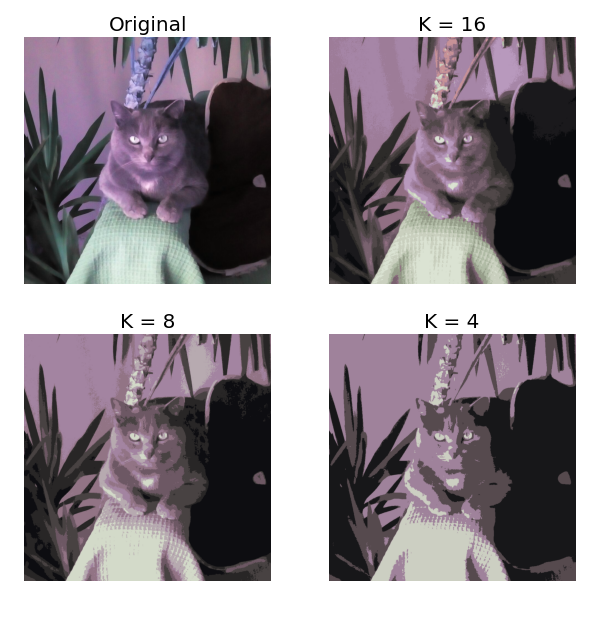
\includegraphics[scale=.3]{ColorQuantization.png}
		\caption{\textit{Color quantized GL image. We observe the original image, a 32 color image which look similar to the original one, a 16 colors image and 8 colors image. Tissue are grouped by color similarity. Reduce the color to the number of cluster will }}\label{fig:ColorQuantization}
	\end{figure}

	Color quantization plays an important role in many application fields such as segmentation, compression, color texture analysis, watermarking, 
	text localization/detection, non photorealistic rendering and content-based retrieval~\cite{ART:Ozturk}.\\
	
	
	Color quantization is used for image segmentation. To this purpose the algorithm aim to reduce the number oin the image is assigned an unique characteristic color. This is the case of medical image segmentation, in which each image color represents a particular characteristic of the tissue displayed (i.e in x-ray represent$\mu$). 
	To perform this technique, different algorithms may be used to group the colors, like clustering algorithm or the principal component analysis.


	
	
	
	

	
	
\end{document}